\documentclass[10pt,A4]{article}

\usepackage{mycv} % load definisi dari mycv.sty

\begin{document}

\pagestyle{fancy}

\vspace{-20.55pt}
\hspace{-0.25\linewidth}\colorbox{bgcol}{\makebox[1.5\linewidth][c]{\HUGE{\textcolor{white}{\textsc{Jan Küster}} } \textcolor{sectcol}{\rule[-1mm]{1mm}{0.9cm}} \HUGE{\textcolor{white}{\textsc{Resume}} } }}

\begin{figure}[H]
\begin{flushright}
	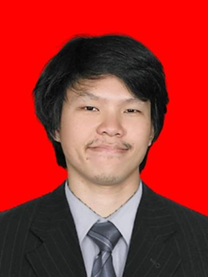
\includegraphics[trim=320 130 460 210,clip,width=0.2\linewidth]{./myfoto.png}
\end{flushright}
\end{figure}

\vspace{-114pt}
\metasection{Status:}{M.Sc. Digital Media, Fullstack JS Engineer}
\metasection{Fields:}{Project Management, Software Development, Consulting} 
\metasection{Tech:}{Meteor, Javascript, Bootstrap, Mongodb, Git, Webstorm, Sourcetree}
\metasection{Loves:}{Global Game Jam, Sci-Fi series, Stackoverflow, Fitness and Martial Arts}

\vspace{6pt}

\cvsection{Experience}
\cvevent{2016 / 09}{Fullstack Javascript Engineer}{University of Bremen}{Invent a realtime classroom management using Meteor and React}{Design software architecture and leading development}
\cvevent{2014 - 2016}{IT Consultant for IBM XPages and Notes Domino}{We4IT GmbH Bremen}{Realize projects in XPages and We4IT Aveedo, monitor project status, conduct reports}{Integrated Camunda BPMN engine and BPMN.IO modeler in We4IT Aveedo}
\cvevent{2012 - 2014}{Scientific Employee / Software Development}{University of Bremen}{Invented a flexible assessment framework, targeting industrial trainees}{Supervised software development lifecycle, Recruited team members}
\cvevent{2011 / 11}{Project Management Simulation Training}{Getoq Consulting}{Performed a two-day project simulation from management perspective}{Topics included customer contracts, change management, controlling, operational tasks}
\cvevent{2010 - 2011}{Student Assistant / Programmer}{otulea.uni-bremen.de}{Realized an online diagnosis platform for workforce literacy development (Flex)}{Modeled software design, implemented various prototypes, conducted usability tests}

\cvsection{Education}
\cvevent{2015 / 07}{Graduated as M.Sc. Digital Media}{University of Bremen}{Master Thesis: Semi Automated Scoring in Technology Based Assessment}{Developed and evaluated an algorithm for semi automated scoring of spreadsheet data}
\cvevent{2012 - 2013}{Master Project - PrIMA}{University of Bremen}{Co-Invented a touch table application for medical support, co-developed software (Java)}{Formed a scrum team, mainted project dev server (Debian), surveyed target audience}
\cvevent{2012 - 2015}{Master Studies Digital Media}{University of Bremen}{Inter-cultural classes in English, covering special topics in computer science and design}{Professionalized in research methods, software development and e-assessment}
\cvevent{2009 - 2010}{Semester Abroad}{University of Melbourne}{Mastered six months of study and trans-cultural experience in Melbourne, Australia}{Finished machine programming, information visualization, professional essay writing}

\null
\vspace*{\fill}
\hspace{-0.25\linewidth}\colorbox{bgcol}{\makebox[1.5\linewidth][c]{\mystrut \small \textcolor{white}{www.jankuester.com} $\cdot$ \textcolor{white}{github.com/jankapunkt}}}

\end{document}
